\documentclass[]{article}
\usepackage[left=1in,top=1in,right=1in,bottom=1in]{geometry}


%%%% more monte %%%%
\usepackage{wrapfig}
% thispagestyle{empty}
% https://stackoverflow.com/questions/2166557/how-to-hide-the-page-number-in-latex-on-first-page-of-a-chapter
\usepackage{color}
% \usepackage[table]{xcolor} % are they using color?

% \definecolor{WSU.crimson}{HTML}{981e32}
% \definecolor{WSU.gray}{HTML}{5e6a71}

% \definecolor{shadecolor}{RGB}{248,248,248}
\definecolor{WSU.crimson}{RGB}{152,30,50} % use http://colors.mshaffer.com to convert from 981e32
\definecolor{WSU.gray}{RGB}{94,106,113}

%%%%%%%%%%%%%%%%%%%%%%%%%%%%

\newcommand*{\authorfont}{\fontfamily{phv}\selectfont}
\usepackage{lmodern}


  \usepackage[T1]{fontenc}
  \usepackage[utf8]{inputenc}




\usepackage{abstract}
\renewcommand{\abstractname}{}    % clear the title
\renewcommand{\absnamepos}{empty} % originally center

\renewenvironment{abstract}
 {{%
    \setlength{\leftmargin}{0mm}
    \setlength{\rightmargin}{\leftmargin}%
  }%
  \relax}
 {\endlist}

\makeatletter
\def\@maketitle{%
  \pagestyle{empty}
  \newpage
%  \null
%  \vskip 2em%
%  \begin{center}%
  \let \footnote \thanks
    {\fontsize{18}{20}\selectfont\raggedright  \setlength{\parindent}{0pt} \@title \par}%
}
%\fi
\makeatother









\title{\textbf{\textcolor{WSU.crimson}{Will Smith Exemplifies Excellence
in Acting}}  }
 

%  

% \author{ \Large true \hfill \normalsize \emph{} }
\author{\Large Rachel
Judd\vspace{0.05in} \newline\normalsize\emph{Washington State University
Vancouver}  }


\date{April 11, 2021}
\setcounter{secnumdepth}{3}

\usepackage{titlesec}
% See the link above: KOMA classes are not compatible with titlesec any more. Sorry.
% https://github.com/jbezos/titlesec/issues/11
\titleformat*{\section}{\bfseries}
\titleformat*{\subsection}{\bfseries\itshape}
\titleformat*{\subsubsection}{\itshape}
\titleformat*{\paragraph}{\itshape}
\titleformat*{\subparagraph}{\itshape}

% https://code.usgs.gov/usgs/norock/irvine_k/ip-092225/


%\titleformat*{\section}{\normalsize\bfseries}
%\titleformat*{\subsection}{\normalsize\itshape}
%\titleformat*{\subsubsection}{\normalsize\itshape}
%\titleformat*{\paragraph}{\normalsize\itshape}
%\titleformat*{\subparagraph}{\normalsize\itshape}

% https://tex.stackexchange.com/questions/233866/one-column-multicol-environment#233904
\usepackage{environ}
\NewEnviron{auxmulticols}[1]{%
  \ifnum#1<2\relax% Fewer than 2 columns
    %\vspace{-\baselineskip}% Possible vertical correction
    \BODY
  \else% More than 1 column
    \begin{multicols}{#1}
      \BODY
    \end{multicols}%
  \fi
}





\usepackage{natbib}
\setcitestyle{aysep={}} %% no year, comma just year
% \usepackage[numbers]{natbib}
\bibliographystyle{./../00-latex-setup/biblio/ormsv080.bst}



\usepackage[strings]{underscore} % protect underscores in most circumstances




\newtheorem{hypothesis}{Hypothesis}
\usepackage{setspace}


%%%%%%%%%%%%%%%%%%%%%%%%%%%%%%%%%%%%%%%%%%%%%%%%%%%%%
%%% MONTE ADDS %%%

\usepackage{fancyhdr} % fancy header 
\usepackage{lastpage} % last page 

\usepackage{multicol}


\usepackage{etoolbox}
\AtBeginEnvironment{quote}{\singlespacing\small}
% https://tex.stackexchange.com/questions/325695/how-to-style-blockquote


\usepackage{soul}			%% allows strike-through
\usepackage{url}			%% fixes underscores in urls
\usepackage{csquotes}		%% allows \textquote in references
\usepackage{rotating}		%% allows table and box rotation
\usepackage{caption}		%% customize caption information
\usepackage{booktabs}		%% enhance table/tabular environment
\usepackage{tabularx}		%% width attributes updates tabular
\usepackage{enumerate}		%% special item environment
\usepackage{enumitem}		%% special item environment

\usepackage{lineno}		%% allows linenumbers for editing using \linenumbers
\usepackage{hanging}


\usepackage{mathtools}  	%% also loads amsmath
\usepackage{bm}		%% bold-math
\usepackage{scalerel}	%% scale one element (make one beta bigger font)

\newcommand{\gFrac}[2]{ \genfrac{}{}{0pt}{1}{{#1}}{#2} }

\newcommand{\betaSH}[3]{  \gFrac{\text{\tiny #1}}{{\text{\tiny #2}}}\hat{\beta}_{\text{#3}}   }
\newcommand{\betaSB}[3]{              ^{\text{#1}} _{\text{#2}} \bm{\beta} _{\text{#3}}                   }  %% bold
\newcommand{\bigEQ}{  \scaleobj{1.5}{{\ }= } }
\newcommand{\bigP}[1]{  \scaleobj{1.5}{#1 } }





\usepackage{endnotes}  % he already does this ...
\renewcommand{\enotesize}{\normalsize}
% https://tex.stackexchange.com/questions/99984/endnotes-do-not-be-superscript-and-add-a-space
\renewcommand\makeenmark{\textsuperscript{[\theenmark]}} % in brackets %
% https://tex.stackexchange.com/questions/31574/how-to-control-the-indent-in-endnotes
\patchcmd{\enoteformat}{1.8em}{0pt}{}{}

\patchcmd{\theendnotes}
  {\makeatletter}
  {\makeatletter\renewcommand\makeenmark{\textbf{[\theenmark]} }}
  {}{}



% https://tex.stackexchange.com/questions/141906/configuring-footnote-position-and-spacing

\addtolength{\footnotesep}{5mm} % change to 1mm

\renewcommand{\thefootnote}{\textbf{\arabic{footnote}}}
\let\footnote=\endnote
%\renewcommand*{\theendnote}{\alph{endnote}}
%\renewcommand{\theendnote}{\textbf{\arabic{endnote}}}


\renewcommand*{\notesname}{ENDNOTES}

\makeatletter
\def\enoteheading{\section*{\notesname
  \@mkboth{\MakeUppercase{\notesname}}{\MakeUppercase{\notesname}}}%
  \mbox{}\par\vskip-2.3\baselineskip\noindent\rule{.5\textwidth}{0.4pt}\par\vskip\baselineskip}
\makeatother


\renewcommand*{\contentsname}{TABLE OF CONTENTS}

\renewcommand*{\refname}{REFERENCES}


%\usepackage{subfigure}
\usepackage{subcaption}

\captionsetup{labelfont=bf}  % Make Table / Figure bold

%%% you could add elements here ... monte says .... %%%
%\usepackage{mypackageForCapitalH}


%%%%%%%%%%%%%%%%%%%%%%%%%%%%%%%%%%%%%%%%%%%%%%%%%%%%%

% set default figure placement to htbp
\makeatletter
\def\fps@figure{htbp}
\makeatother


% move the hyperref stuff down here, after header-includes, to allow for - \usepackage{hyperref}

\makeatletter
\@ifpackageloaded{hyperref}{}{%
\ifxetex
  \PassOptionsToPackage{hyphens}{url}\usepackage[setpagesize=false, % page size defined by xetex
              unicode=false, % unicode breaks when used with xetex
              xetex]{hyperref}
\else
  \PassOptionsToPackage{hyphens}{url}\usepackage[draft,unicode=true]{hyperref}
\fi
}

\@ifpackageloaded{color}{
    \PassOptionsToPackage{usenames,dvipsnames}{color}
}{%
    \usepackage[usenames,dvipsnames]{color}
}
\makeatother
\hypersetup{breaklinks=true,
            bookmarks=true,
            pdfauthor={Rachel Judd (Washington State University
Vancouver)},
             pdfkeywords = {Will Smith; Denzel Washington; excellence in
acting},  
            pdftitle={Will Smith Exemplifies Excellence in Acting},
            colorlinks=true,
            citecolor=blue,
            urlcolor=blue,
            linkcolor=magenta,
            pdfborder={0 0 0}}
\urlstyle{same}  % don't use monospace font for urls

% Add an option for endnotes. -----

%
% add tightlist ----------
\providecommand{\tightlist}{%
\setlength{\itemsep}{0pt}\setlength{\parskip}{0pt}}

% add some other packages ----------

% \usepackage{multicol}
% This should regulate where figures float
% See: https://tex.stackexchange.com/questions/2275/keeping-tables-figures-close-to-where-they-are-mentioned
\usepackage[section]{placeins}



\pagestyle{fancy}   
\lhead{\textcolor{WSU.crimson}{\textbf{ Will Smith Exemplifies
Excellence in Acting }}}
\chead{}
\rhead{\textcolor{WSU.gray}{\textbf{  Page\ \thepage\ of\ \protect\pageref{LastPage} }}}
\lfoot{}
\cfoot{}
\rfoot{}


\begin{document}
	
% \pagenumbering{arabic}% resets `page` counter to 1 
%    

% \maketitle

{% \usefont{T1}{pnc}{m}{n}
\setlength{\parindent}{0pt}
\thispagestyle{plain}
{\fontsize{18}{20}\selectfont\raggedright 
\maketitle  % title \par  

}

{
   \vskip 13.5pt\relax \normalsize\fontsize{11}{12} 
   
\textbf{\authorfont Rachel Judd} \hskip 15pt \emph{\small Washington
State University Vancouver}   

}

}








\begin{abstract}

    \hbox{\vrule height .2pt width 39.14pc}

    \vskip 8.5pt % \small 

\noindent Will Smith is a better actor than Denzel Washington. This is
seen through how many millions of dollars his movies earned, how short a
time he has taken to reach his level of success, the height of his
ratings, the variety of genres he has acted in, and the amount of votes
his movies have received.


\vskip 8.5pt \noindent \textbf{\underline{Keywords}:} Will Smith; Denzel
Washington; excellence in acting \par

    




    
    \hbox{\vrule height .2pt width 39.14pc}
    \vskip 5pt 
    \hfill \textbf{\textcolor{WSU.gray}{ April 11, 2021 } }
    \vskip 5pt 
    
\end{abstract}


\vskip -8.5pt



 % removetitleabstract

\noindent  

\begin{figure}[!ht]
 \label{fig:one-graphic}
%% figures have hrule, tables have hline
    \begin{center}
        \scalebox{1.00}{    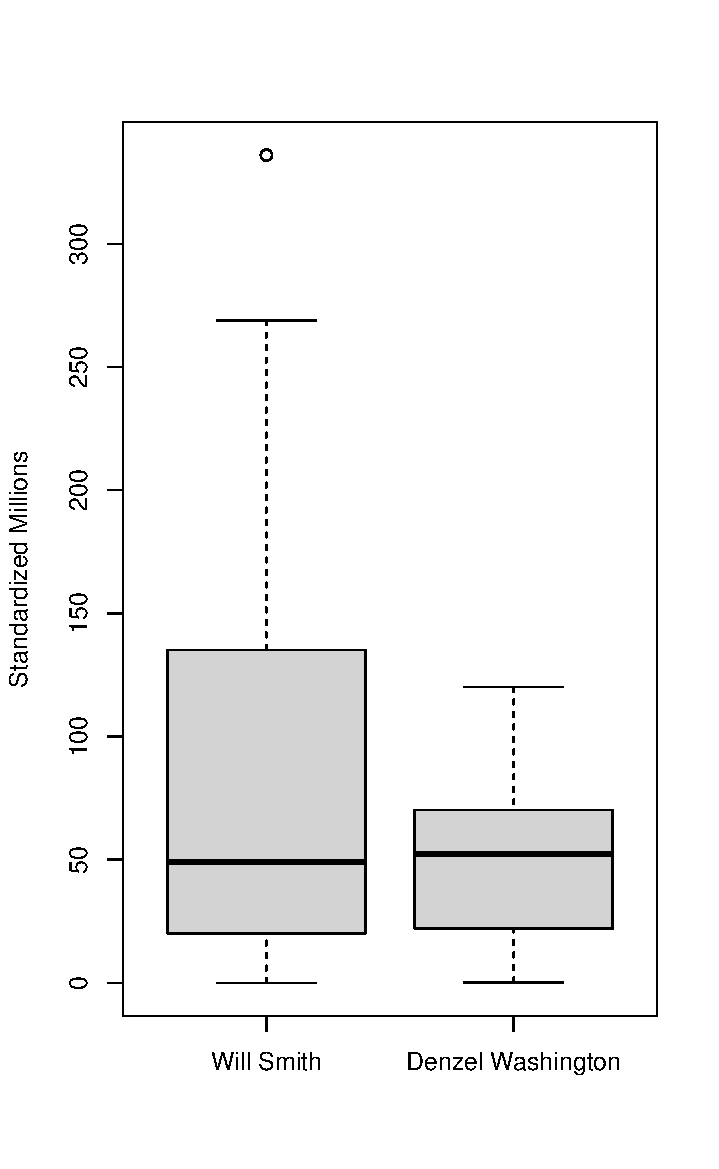
\includegraphics[trim = 0 50mm 0 5mm,clip,width=\textwidth]{figures/will=better-sd-millions2000.pdf} }
    \end{center}
    \hrule
      \vspace{2mm}
    \caption{ \textbf{Will Smith's movies have earned more than those of Denzel Washington:} \newline \footnotesize{ This graph shows the millions of dollars earned for both Will Smith's movies and for Denzel Washington's movies.  \newline \newline  The dollar amounts were standardized to avoid the influence of inflation. The amount was scaled to what the amount would be in the year 2000. }  }
    \vspace{2mm}
    \hrule
\end{figure}

\section{Introduction}
\label{sec:intro}

\doublespacing

There are several ways to measure success as an actor, including votes,
millions earned, ratings, and the number of genres in which the actor
has acted. The votes show how well-liked the actor's movies are, with
more votes reflecting superior acting performance. The millions of
dollars each movie earns is an important measure of an actor's success.
Higher earnings reflect better performance. The earnings for the
excellent actor's movies will accumulate faster than the earnings for a
less successful actor. High ratings also reflect excellent acting. The
number of genres acted in is another valuable measure of excellence in
acting. The ability to act in mulitiple genres demonstrates flexibility
and a higher level of skill than just acting in one genre.

Will Smith has demonstrated excellence in acting through his high
ratings, high number of votes, the millions of dollars his movies have
earned, and his versatility in the genres in which he can act. On these
dimensions, he has shown that he is a superior to other actors, such as
Denzel Washington.

\newpage
\section{ Comparison to Denzel Washington}
\label{sec:da}

Will Smith has outperfomred Denzel Washington in a variety of measures
of excellence. The most votes Smith has received for a film is 675,160,
43\% more than Washington's maximum amount of votes (383,980). Smith's
average amount of votes is 131,488, which is 18467 votes more than
Washington's average amount of votes.

The millions of dollars Smith's movies have earned (standardized to the
year 2000) also show Smith's acting excellence. The highest one of
Smith's movies has earned is 336.026 million dollars, 64\% more than the
highest a Denzel Washington movie has earned. Smith's mean earnings are
also 40\% more than that of Washington, at 81.87 million dollars.
Smith's movies have earned a total of 4,256.99 million dollars, which he
earned in only 29 years, compared to Washington's 2,340.43 million
dollar earnings in 40 years. These high earnings in such a short period
of time show Smith's excellence in acting.

Smith's films have also received higher ratings than Washington's. The
highest rating Smith has received is 8.6, with a median rating of 6.3.
These high ratings show superior acting performance.

Smith is also a more versatile actor than Washington. Smith has acted in
18 different genres, 11\% more than Washington. Smith has acted in more
movies in the genres of action, adventure, animation, comedy,
documentary, drama, family, fantasy, musical romance, and sci-fi than
Washington has, with a maximum difference of 87\%.

\section{ Conclusion}
\label{sec:conclusion}

The assessment of excellence in acting requires multiple measures
including votes received, ratings, millions of dollars earned, the
amount of time it took to accumulate those earnings, and the number of
genres acted in. These measures work together to show how well-liked the
actor's movies are, the monetary value of these movies, and the actor's
versatiliy. On each of these dimensions, Will Smith has shown himself
superior to actors like Denzel Washington, exemplifying excellence in
acting.




%% appendices go here!


\newpage
\theendnotes

%%%%%%%%%%%%%%%%%%%%%%%%%%%%%%%%%%%  biblio %%%%%%%%
\newpage
\begin{auxmulticols}{1}
\singlespacing 
\bibliography{./../00-latex-setup/biblio/master.bib}

%%%%%%%%%%%%%%%%%%%%%%%%%%%%%%%%%%%  biblio %%%%%%%%
\end{auxmulticols}

\newpage
{
\hypersetup{linkcolor=black}
\setcounter{tocdepth}{3}
\tableofcontents
}



\end{document}